\documentclass[../tesis.tex]{subfiles}
\graphicspath{{\subfix{../images/}}}
\begin{document}
El presente capítulo detalla las fuentes de datos y el procesamiento de los mismos y las métricas utilizadas para los experimentos realizados. Éstos, a continuación, se describen en detalle, tanto los modelos utilizados como descripciones de las construcción, entrenamiento y evaluación de mismo.


\section{Fuente de datos}
El origen de los datos que son utilizados en los experimentos se basan en el primer sondeo de PanSTARRS (DR1) \cite{panstarrs}. Éstos datos consisten en información capturada del cielo en forma de imágenes a través del telescopio PanSTARRS en cinco bandas las cuales son: $g$, $r$, $i$, $z$, $y$ conocidas como $grizy$. Son almacenados en la \textit{Space Telescope Science Institute} (STScI) y disponibilizados en la plataforma de Mikulski Archive for Space Telescopes (MAST). Existen herramientas de automatización ofrecidas por investigadores para obtener los datos del telescopio. En particular, en este trabajo se utiliza las librerías de Python llamadas $panstamps$ y $hips2fits$ para descargar las imágenes mediante un script y almacenarlas en los servidores de \textbf{ALeRCE}.\par\null\par

A través de estas herramientas, se puede descargar imágenes a partir de coordenadas ecuatoriales (declinación y ascensión recta), por lo que la extracción de datos se basa en seleccionar las galaxias anfitrionas candidatas a transitorios y buscar las imágenes en PanSTARRS en base a las coordenadas del transitorio.\par\null\par

Para esto, el equipo de \textbf{ALeRCE} generó dos muestras, descritos a continuación

\begin{enumerate}
    \item \textbf{Muestro de ALeRCE:} Compuesta por $14,111$ galaxias anfitrionas candidatas a transitorios identificadas visualmente por el equipo de brokers de ALeRCE entre agosto de 2019 y mayo de 2022. El flujo de identificación inicia con la clasificación de las alertas publicas de la \textit{Zwicky Transient Facility} (ZTF). Luego son filtrados mediante la herramienta ALeRCE SN Hunter. Los candidatos resultantes se utilizaron para seleccionar visualmente la posición más probable de la galaxia anfitriona entre las posiciones de la \textit{NASA Extragalactic Database} (NED, Helou et al. 1991); \textit{Set of Identifications, Measurements and Bibliography for Astronomical Data} (SIMBAD, Wenger et al. 2000); y las fuentes del \textit{Sloan Digital Sky Survey} (SDSS, Abdurro’uf et al. 2022) superpuestas en imágenes a color de PanSTARRS DR1 usando la herramienta ipyaladin.

    \item \textbf{Muestra cercana:} Compuesta por $2,563$ galaxias anfitrionas identificadas visualmente del catálogo de \textit{Asiago} (Barbon et al. 1999) y $117$ galaxias anfitrionas que tienen supernovas (SNe) reportadas en la \textit{Transient Name Server} (TNS) en el catálogo \textit{HECATE} (Kovlakas et al. 2021) de galaxias cercanas.
\end{enumerate}

Finalmente, las galaxias anfitrionas candidatas a transitorios son localizadas usando las coordenadas ecuatoriales del transitorio y descargadas desde PanSTARRS.\par\null\par

En total, $16,791$ galaxias componen el conjunto de datos, las cuales corresponden a galaxias anfitrionas cuyos eventos transitorios candidatos estén dentro de un radio de un arco minuto desde el centro de la galaxia anfitriona.\par\null\par

\subsection{Imágenes de la banda r de PanSTARRS DR1 mediante panstamp} \label{methods:dataset1}
Por cada galaxia anfitriona candidata a transitorio, se obtiene una imagen de dimensiones $480\times480$ píxeles con $0.25^{\prime\prime}$ por pixel, centrado en la posición del transitorio.\par\null\par

\subsection{Imágenes de las bandas grizy de PanSTARRS DR1 mediante hips2fits}\label{methods:dataset2}
Al igual que el set de datos anterior, por cada galaxia anfitriona candidata  a transitorio se obtiene una imagen de cada banda, de tamaño $480\times480$ píxeles con $0.25^{\prime\prime}$ por píxel centrado en la posición del transitorio. Éstas imágenes contienen un preprocesado por parte de la herramienta que las hace más ruidosas, y por ende, distintas a las imágenes obtenidas mediante $panstamps$, es por esto que el presente trabajo las considera como dos fuentes de datos distintas.\par\null\par

\begin{figure}[h]
\centering
\begin{subfigure}{.5\textwidth}
  \centering
  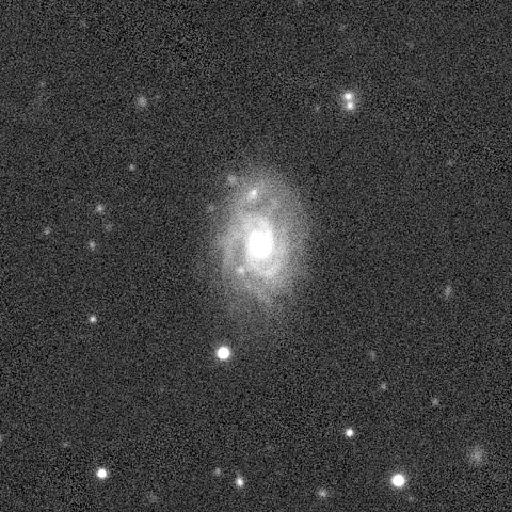
\includegraphics[width=0.89\linewidth]{images/ZTF18aarunub_panstamps_r.jpeg}
  \label{fig:ZTF18aarunub_panstamps_r}
\end{subfigure}%
\begin{subfigure}{.5\textwidth}
  \centering
  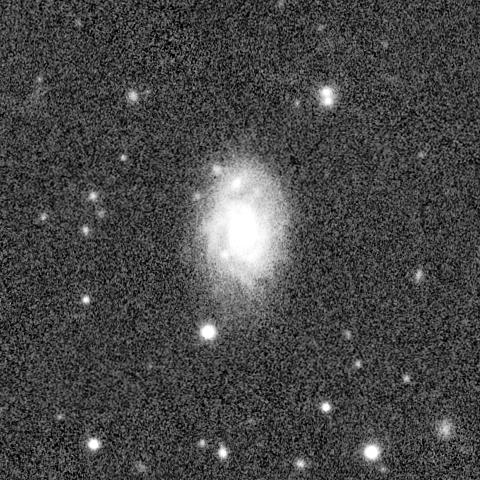
\includegraphics[width=0.9\linewidth]{images/ZTF18aarunub_hips2fits_r.jpg}
  \label{fig:ZTF18aarunub_hips2fits_r}
\end{subfigure}
\caption{Ejemplo de diferencias entre las herramienta $panstamps$ (a la izquierda) y la herramienta $hips2fits$ (a la derecha) para la galaxía ZTF18aarunub en la banda $r$ usando la misma posición espacial.}
\label{fig:test}
\end{figure}

\section{Procesamiento de las imágenes}\label{methods:process}
En ambas fuentes de datos se utiliza las estrategias de limpieza y generación de imágenes multiresolución detallados en el trabajo de \cite{delight}, las cuales se pueden resumir en tres partes:\par\null\par

\begin{enumerate}
    \item \textbf{Eliminación de ruido:} Consiste en un procesado a las imágenes usando SExtractor con la herramienta SEP \cite{sex} para restar la emisión del cielo y detectar fuentes significativas
    \item \textbf{Imágenes Multiresolución:} Consiste en la creación de un conjunto de cinco imágenes multiresolución. Esto obliga a que la entrada sea una representación más compacta de los datos, permitiendo su inclusión directa en futuras alertas enriquecidas. Todas las imágenes están centradas alrededor de la posición del transitorio y tienen el mismo tamaño en píxeles; son imágenes cuadradas con lado de $480/2^4$ píxeles, pero tienen diferentes campos de visión, con lados $120^{\prime\prime}/2^{i-1}$ con $i \in 1..5$, yendo de escalas más grandes a más pequeñas. Los píxeles del nivel $i$ pueden construirse tomando el promedio de $2\times2$ píxeles a la resolución del nivel $i + 1$.
    \item \textbf{Normalización:} Consiste en la normalización entre cero y uno utilizando los valores mínimos y máximos entre todos los niveles de un objeto dado.
\end{enumerate}

\begin{figure}[h]
    \centering
    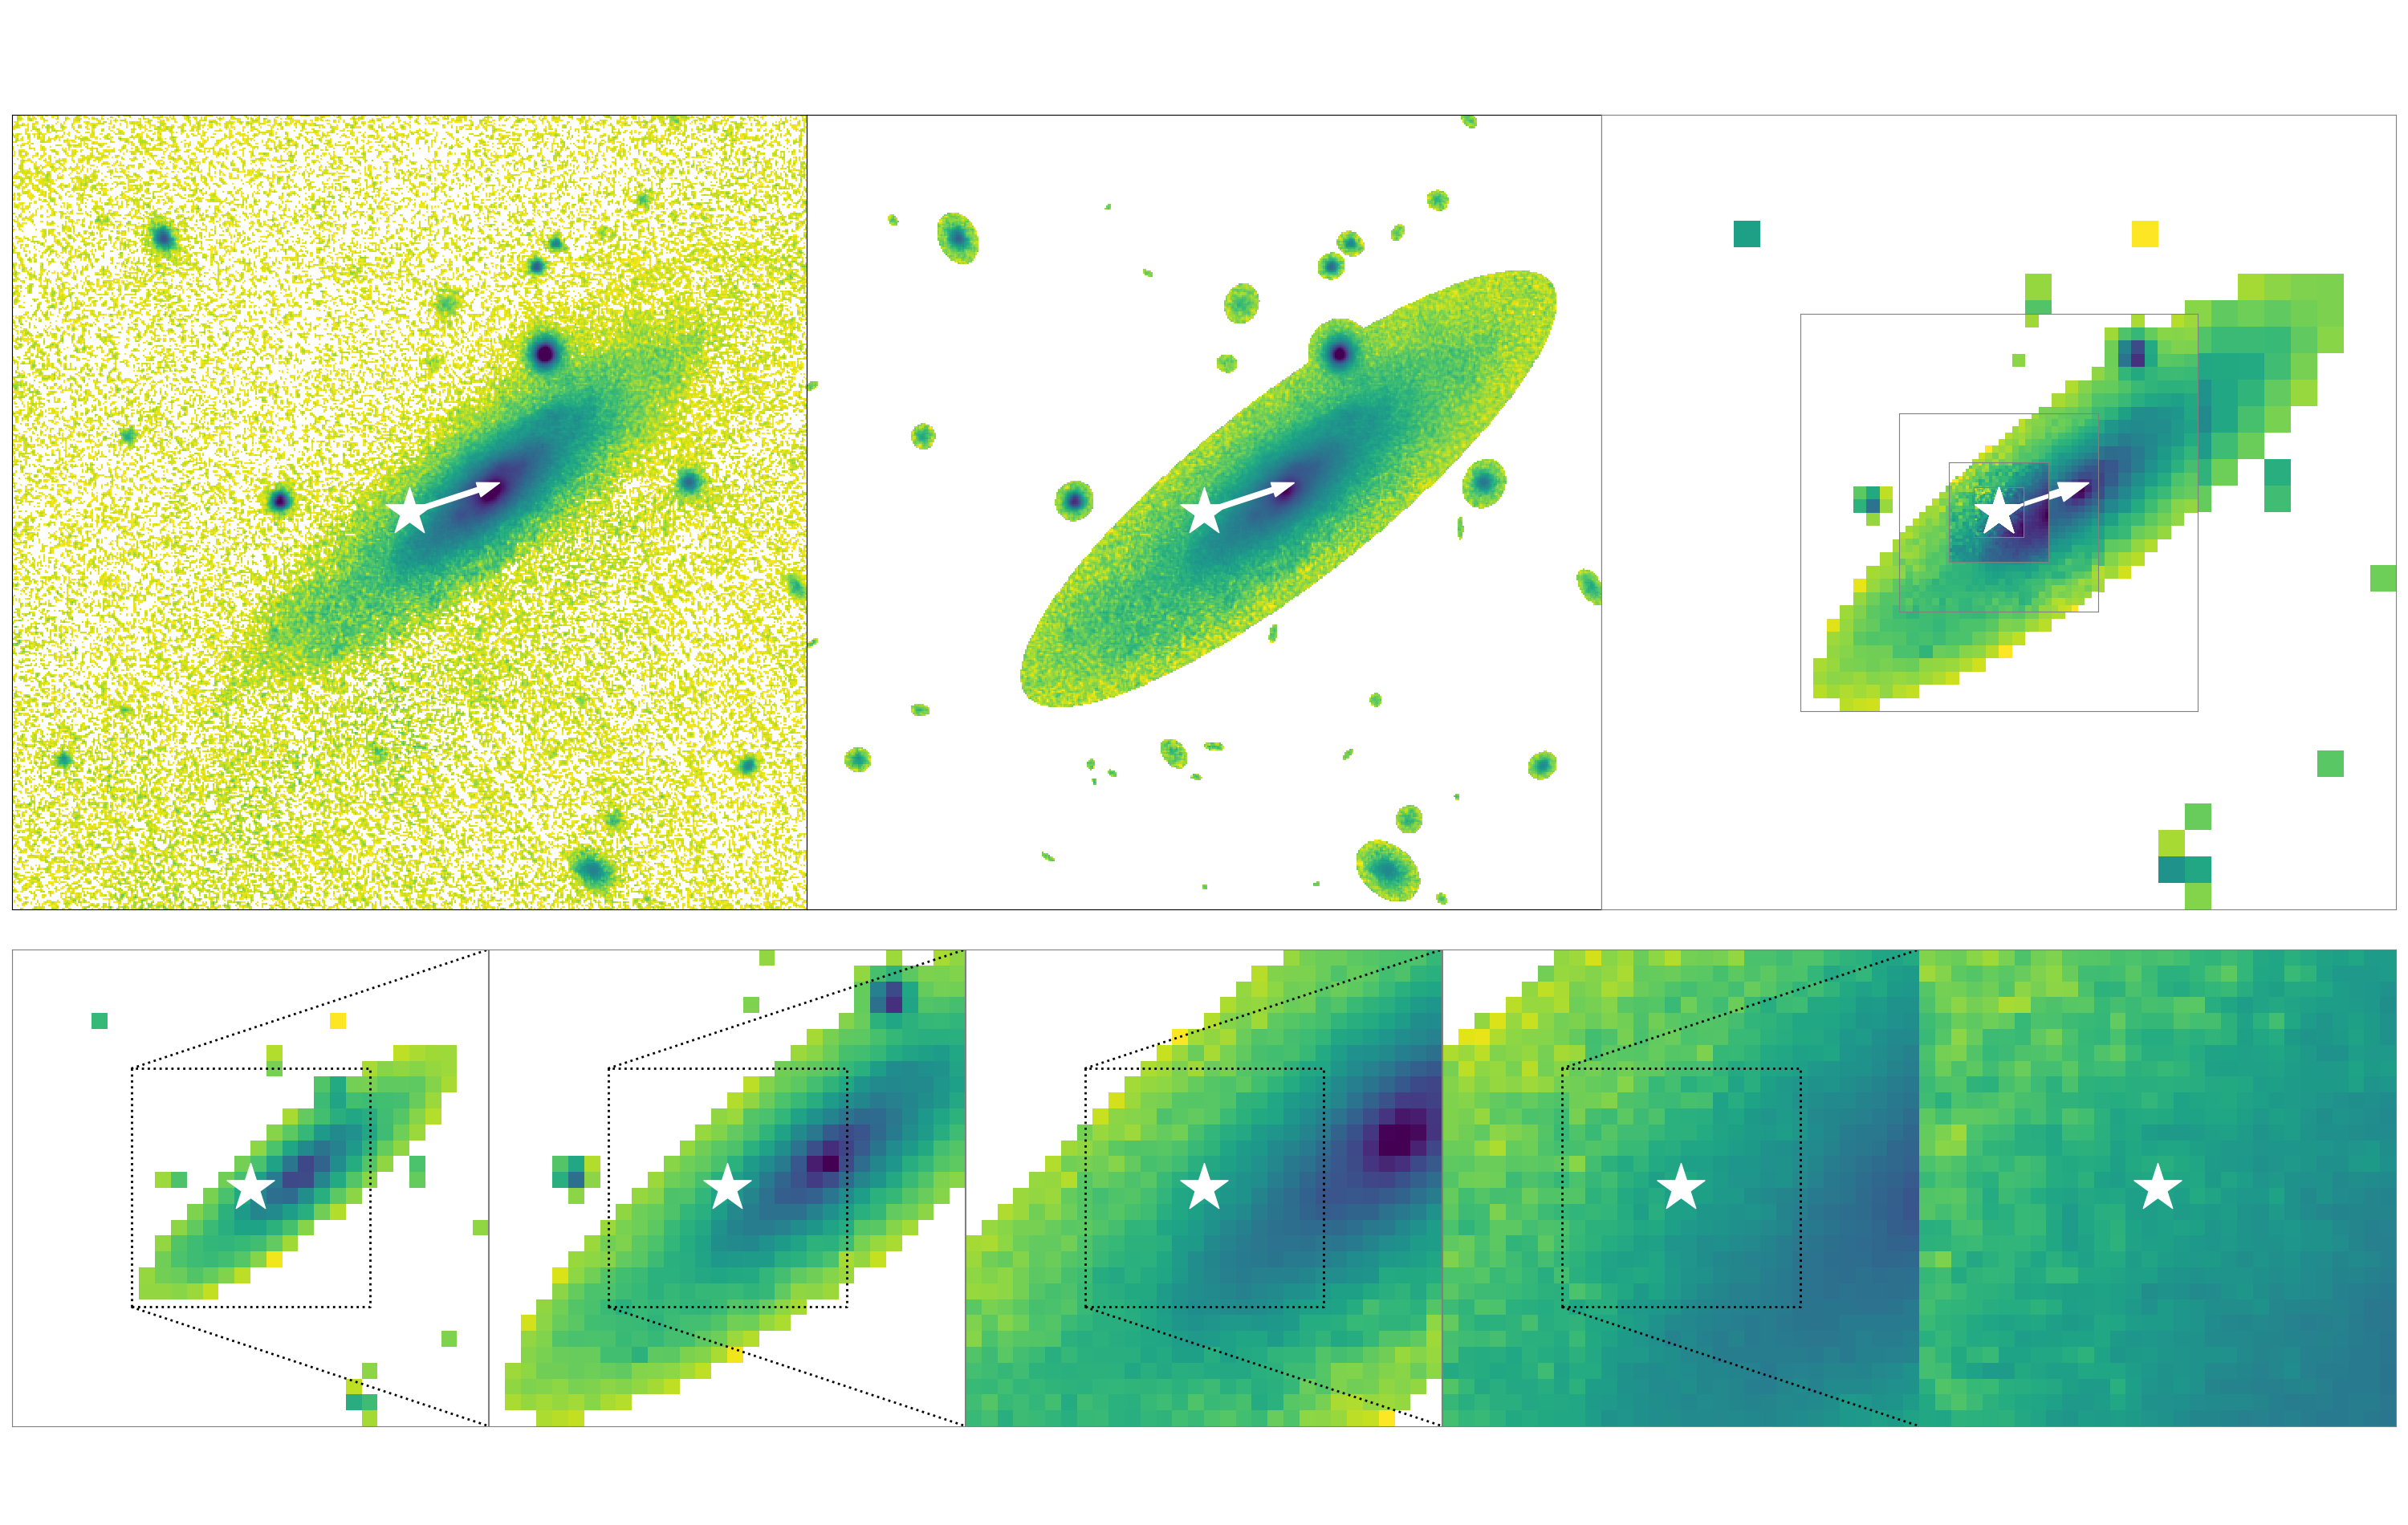
\includegraphics[width=1\linewidth]{images/ZTF19aczjytt_comp.png}
    \caption{Etapas del procesado de las imágenes obtenidas de PanSTARRS. En la primera fila, se observa la imágen original, la imagen posterior a la eliminación del ruido provocado por las emisiones y la imagen con las cinco multiresoluciones a generar. En la segunda fila se observa las multiresoluciones ya generadas. La flecha conecta al transitorio (estrella) y el centro de la galaxia anfitriona (punta de flecha)}
    \label{fig:process-summarization}
\end{figure}

\section{Métricas}\label{methods:metrics}

En este trabajo se emplean las siguientes métricas para evaluar el rendimiento del modelo:

\begin{equation}\label{eq:mse}
MSE = \frac{1}{n} \sum_{i=1}^{n} (Y_i - \hat{Y}_i)^2
\end{equation}

\begin{equation}\label{eq:rmse}
RMSE = \sqrt{MSE} = \sqrt{\frac{1}{n} \sum_{i=1}^{n} (Y_i - \hat{Y}_i)^2}
\end{equation}

\begin{equation}\label{eq:mean_deviation}
\textit{Desviación Media} = \frac{1}{n} \sum_{i=1}^{n} \| Y_i - \hat{Y}_i \|
\end{equation}

\begin{equation}\label{eq:median_deviation}
\textit{Desviación Mediana} = \text{mediana}(\| Y_i - \hat{Y}_i \|)
\end{equation}

\begin{equation}\label{eq:mode_deviation}
\textit{Desviación Moda} = \text{moda}(\| Y_i - \hat{Y}_i \|)
\end{equation}

Donde:
\begin{itemize}
    \item $n$: Es el tamaño total de los datos para un conjunto arbitrario.
    \item $Y$: Es un conjunto de puntos 2D de tamaño $n$ que representa la posición real de la galaxia anfitriona. $Y = \{(x_1, y_1), (x_2, y_2), \ldots, (x_n, y_n)\}$, $Y_i = (x_i, y_i) \in Y$
    \item $\hat{Y}$: Es un conjunto de puntos 2D de tamaño $n$ que representa la posición predicha de la galaxia anfitriona. $\hat{Y} = \{(\hat{x_1}, \hat{y_1}), (\hat{x_2}, \hat{y_2}), \ldots, (\hat{x_n}, \hat{y_n})\}$, $\hat{Y}_i = (\hat{x_i}, \hat{y_i}) \in \hat{Y}$
\end{itemize}

A continuación, en base a los objetivos de este trabajo, se busca realizar cuatro principales experimentos, que consisten en el desarrollo de distintos modelos para explorar la reproducibilidad, multimodalidad de los algoritmos y su capacidad de transferencia del aprendizaje.\par\null\par

Todos los experimentos se realizan en el ecosistema de \textit{Python}, utilizando la librería \textit{PyTorch}. La elección de la herramienta responde a la necesidad del equipo de \textbf{ALeRCE} de tener todos sus modelos implementados en dicha librería, y se espera que los resultados del presente trabajo sean utilizados por el equipo en sus entornos de producción.\par\null\par

\section{Experimento 1: Reproducibilidad de resultados} \label{methods:replication}
Se busca reproducir los resultados del trabajo de \cite{delight} y extenderlo para usarse como base en los siguientes experimentos. Sin embargo, para replicar la arquitectura de \textbf{DELIGHT} en el entorno de PyTorch, se propone realizar algunas modificaciones y optimizaciones para hacer más extensible el modelo y reducir los tiempos de entrenamiento.\par\null\par

\subsection{Modelo propuesto: DelightPt}

Una primera modificación es la entrada del modelo, que originalmente recibe un tensor de $B\times L\times30\times30$, que representa un lote de $B$ imágenes de dimensiones $L\times30\times30$ correspondientes a las $L$ resoluciones analizadas en la sección \ref{methods:process}. Se propone la implementación de una capa de entrada de dimensiones $B\times L\times C\times W\times H$, donde $B$ es el batch, $L$ son las resoluciones, $C$ son los canales de la imagen, y $W,H$ sus dimensiones. Así, una imagen de dimensiones $B\times5\times1\times30\times30$ es equivalente a la capa de entrada del modelo \textbf{DELIGHT}.\par\null\par

El modelo realiza una serie de rotaciones y volteos de la imagen, con el fin de hacerlo robusto a estas transformaciones. Como se revisó en la sección \ref{introduction:delight}, a partir del conjunto de cinco imágenes se generan ocho transformaciones para cada una de ellas, obteniéndose un total de cuarenta imágenes. A su vez, la sección convolucional comparte los pesos, y procesa cada imagen por separado. Es decir, para las cuarentas imágenes resultantes de la sección de transformación, se generan cuarenta vectores de características. Finalmente, la sección de regresión recibe la concatenación de cinco vectores de características que representan las cinco resoluciones de una imagen y retorna una posición. Es decir, de los cuarenta vectores de la sección anterior, se debe crear ocho grupos de cinco vectores cada uno, donde un grupo corresponde a una transformación y los vectores pertenecientes al grupo corresponden a las resoluciones. Por lo tanto, se busca generar un tensor de dimensiones tales que sea compatible con la operación de convolución de PyTorch, el cual recibe como entrada un tensor de dimensiones $B\times C\times W \times H$, y así aprovechar el paralelismo que ofrece este entorno de trabajo, disminuyendo no solo el tiempo de entrenamiento, sino el tiempo de inferencia.\par\null\par

Para esto, el experimento propone concatenar cada transformación dentro de la dimensión $B$, es decir, si recibimos una entrada de dimensiones $B\times L\times C\times W\times H$, se genera una salida de dimensiones $(B \cdot T \cdot L)\times C\times W\times H$, con $T$ la cantidad de transformaciones efectuadas ($T=8$ en \textbf{DELIGHT}). La concatenación está ordenada, es decir, si consideramos una imagen cualquiera $X^{b_i}_{{t_j}{t_l}}$ con $b_i$ el lote $i$-esimo, $t_j$ la transformación $j$-esima y $l_k$ la resolución $k$-esima , $i,j,k \in \{1...n\}$, el orden de los elementos en $(B \cdot L \cdot T)\times C\times W\times H$ es $\{X^{b_1}_{{t_1}{l_1}}, X^{b_1}_{{t_1}{l_2}}, ..., X^{b_1}_{{t_1}{l_n}}, X^{b_1}_{{t_2}{l_1}}, ..., X^{b_1}_{{t_2}{l_n}}, ..., X^{b_1}_{{t_n}{l_n}}, ..., X^{b_n}_{{t_n}{l_n}}\}$. Esto es equivalente a haber ordenado por lote, luego por transformación, y finalmente por resolución. Así, el tensor resultante de dimensiones $(B \cdot T \cdot L)\times C\times W\times H$ es compatible con la entrada de la operación de convolución de PyTorch de dimensiones $B\times C\times W \times H$.\par\null\par

Finalmente, se debe deshacer la concatenación en dos partes, primero dividiendo el conjunto de imágenes en la cantidad de lotes $B$, y luego en la cantidad de transformaciones $T$, concatenando los vectores de características de las $L$ resoluciones generadas a partir de una imagen. Esta operación es equivalente a transformar un tensor de dimensiones $(B \cdot T \cdot L)\times F$ con $F$ la cantidad de características generadas de la convolución, a un tensor de dimensiones $(B \times T \times (L \cdot F))$. Éste último tensor es compatible con la sección de regresión, generando una salida de dimensiones $B \times T \times 2$, que, al aplicarse una reorientación (reshape) de los índices, se obtiene una salida de dimensiones $B \times (T \cdot 2)$, equivalente al vector salida de \textbf{DELIGHT}\par\null\par

\subsection{Entrenamiento}
En el entrenamiento, se utiliza la herramienta Ray Tune \cite{raytune} para la búsqueda de hiper parámetros a escoger para la arquitectura de la red, empleando la estrategia de búsqueda de hiper parámetros planteada en el trabajo de \cite{delight}. Las $16,791$ imágenes se dividen en conjuntos de entrenamiento, validación y evaluación. El conjunto de entrenamiento se compone de $9,605$, el de validación de $2,402$ y el de evaluación de $4,784$ imágenes. El entrenamiento se compone de dos modos: desarrollo y producción.\par\null\par

El modo de desarrollo contiene un conjunto de entrenamiento de $16.630$ imágenes, obtenidas realizando un balanceo de clases del conjunto original de $9,605$ imágenes. Dicho balanceo se obtiene al nivelar las clases de imágenes de los candidatos a transitorio provenientes del ZTF y de Asiago explicados en la sección \ref{methods:dataset1}. A su vez, el conjunto de validación es filtrado, seleccionando las imágenes cuya galaxia anfitriona se encuentre dentro de un radio de $60$ píxeles.\par\null\par

El modo de producción descarta los balanceos y filtros, y concatena el conjunto de entrenamiento con el de validación, siendo éste un nuevo conjunto de entrenamiento de $12,007$ imágenes. El conjunto de validación es ahora el conjunto de evaluación, compuesta por $4,784$\par\null\par

En ambos modos, el optimizador utilizado es Adam \cite{adam} con una tasa de aprendizaje de $0.0014$ y un regularizador por \textit{weight decay} de $0.0001$. El valor de \textit{dropout} para la sección de regresión es del 6\%, el tamaño de lotes es $40$ (\textit{batch size}), y la función de error es el error cuadrático medio (MSE). El entrenamiento utiliza $20$ épocas en el modo de desarrollo, y $100$ épocas en el modo de producción.\par\null\par

\subsection{Evaluación}
El modelo final, entrenado en el modo de producción, se evalúa en el conjunto de evaluación, utilizando cuatro métricas descritas en la sección \ref{methods:metrics} las cuales corresponden a la raiz de la MSE, la distancia media, mediana y moda. Éstas métricas son las utilizadas para comparar con el modelo \textit{baseline}, \textbf{DELIGHT}.

\section{Experimento 2: Arquitecturas preentrenadas}\label{methods:pretrained_arc}
El uso de arquitecturas que han sido preentrenadas en conjuntos de millones de datos genera un sin fin de oportunidades de estudio. En lo que respecta a este trabajo, la viabilidad de utilizar las características generadas por una fuente de datos genérica como ImageNet abre la posibilidad de utilizar arquitecturas más flexibles, como Vision Transformers \cite{ViT}, que permitiría incorporar no solo imágenes, sino curvas de luz, espectrogramas, entre otros. El poder contar con un modelo multimodal de estas características permitiría solucionar el problema de clasificar un evento transitorio directamente de las fuentes de datos primarias, ganando tiempo y recursos vitales para la recopilación de datos alrededor de los eventos de interés.\par\null\par

Por esta razón, el presente trabajo estudia la capacidad de generalización de modelos preentrenados. En particular para este caso de estudio, el trabajo se centra en estudiar la capacidad de generalización de modelos preentrenados en ImageNet \cite{imagenet}. La elección de este \textit{pretrained} se basa en la amplia disponibilidad de arquitecturas preentrenadas en dicha fuente de datos, y en particular, existen ejemplos en la literatura que ya han utilizado modelos preentrenados en ImageNet para tareas astronómicas, principalmente de clasificación de galaxias \cite{galaxytransferlearning}.\par\null\par

La arquitectura utilizada para el estudio es Resnet50 \cite{resnet}. La elección en contraste con Vision Transformers responde a la necesidad de tiempos de inferencias más cortos, sacrificando precisión. Esto es posible dado que el motivo central de este estudio es el evaluar ImageNet como generalizador para la tarea de \textbf{DELIGHT}, lo que lo hace independiente a la arquitectura escogida.\par\null\par

Dado que Resnet50 recibe como entrada una imagen de dimensiones $3\times224\times224$, se debe buscar una transformación de las imágenes multiresolución de entrada $5\times1\times30\times30$ a $3\times224\times224$. El problema de lo anterior es que ésto agrega más variabilidad a los experimentos. Es por esto que en este trabajo se decide utilizar las imágenes originales de la fuente de datos descrita en la sección \ref{methods:dataset1} repitiendo la información entre canales para construir una imagen en blanco y negro, reemplazando el procesamiento detallado en la sección \ref{methods:process} por la combinación de un cambio de tamaño usando una interpolación bilineal desde $3\times480\times480$ a $3\times256\times256$, un recorte central de tamaño $224$ con una imagen resultante de $3\times224\times224$, un reescalado $[0, 1]$ de los datos de la imagen, y una normalización utilizando como promedio $(0.485, 0.456, 0.406)$ por canal, con desviación estandar $(0.229, 0.224, 0.225)$ por canal. Así, la imagen resultante es compatible con la capa de entrada de Resnet50.\par\null\par

Los experimentos consisten en evaluar tres variaciones del modelo de Resnet50: Delight Resnet50 (\textit{DR50}), Delight Resnet50 utilizando la estrategia de Fine Tuning preentrenado en ImageNet (\textit{DR50FT+ImageNet}) y Delight Resnet50 utilizando la estrategia de Feature Extration a partir de ImageNet (\textit{DR50FE+ImageNet}). Las tres variaciones comparten la misma arquitectura, pero varían en la estrategia de entrenamiento. La arquitectura se compone de dos elementos principales, un generador de características y una sección de regresión. El generador de características, el cual denominaremos como \textit{backbone}, corresponde a modificar la salida de Resnet50 para que finalice su computo después de las capas convolucionales, sin pasar por las capas \textit{fully-connected}, éste vector resultante son las características de la imagen de entrada. Finalmente, el vector resultante se conecta a una sección de regresión, compuesta por una capa densa con función de activación $Tanh$, una capa de \textit{dropout} y una capa densa de salida $B\times2$.\par\null\par


\subsection{Modelo propuesto I: DR50}
Esta estrategia consiste en un \textit{backbone} no entrenado, es decir, se inicializa los pesos del \textit{backbone} en vez de utilizar los pesos correspondientes al preentrenamiento con ImageNet. Así, se utiliza este modelo como \textit{baseline} para los experimentos siguientes.

\subsection{Modelo propuesto II: DR50FT+ImageNet}
Se busca un \textit{backbone} con los pesos correspondientes al preentrenamiento con ImageNet. Se deja activados los gradientes del \textit{backbone} de tal forma que en el entrenamiento todos los pesos de la red serán actualizados. Se busca así evaluar si un \textit{fine tuning} basado en ImageNet logra generalizar la tarea.

\subsection{Modelo propuesto III: DR50FE+ImageNet}
En este último experimento, se utiliza un \textit{backbone} con los pesos correspondientes al preentrenamiento con ImageNet. Sin embargo, se desactivan los gradientes del mismo, es decir, en el entrenamiento sólo los pesos de la sección de regresión serán actualizados. El objetivo de éste experimento es evaluar si un \textit{feature extration} es suficiente para generalizar la tarea.

\subsection{Entrenamiento}
Para el entrenamiento se reutiliza la estrategia de la sección \ref{methods:replication} con respecto a los modos de desarrollo y producción. El optimizador escogido es Adam \cite{adam} con una tasa de aprendizaje de $0.0014$ y un regularizador por \textit{weight decay} de $0.0001$. El valor de \textit{dropout} para la sección de regresión es del 50\%, el tamaño de lotes es $40$ (\textit{batch size}), y la función de error es el error cuadrático medio (MSE). El entrenamiento utiliza $20$ épocas en el modo de desarrollo, y $100$ épocas en el modo de producción.\par\null\par

\subsection{Evaluación}
Se reutiliza la evaluación propuesta en la sección \ref{methods:replication}.

\section{Experimento 3: Multimodalidad}\label{methods:multimodality}
El trabajo de \cite{delight} se limita al uso de los datos descritos en la sección \ref{methods:dataset1}, por lo que este trabajo experimenta el desempeño del algoritmo \textbf{DELIGHT} si se incorporasen la información de las bandas $grizy$ descritas en la sección \ref{methods:dataset2}. 

\subsection{Modelo propuesto: DelightPtMultiband}
La modificación de la capa de entrada a un tensor de dimensiones $B\times L\times C\times W\times H$ propuesta en el primer experimento permite estudiar el caso para imágenes de más de un canal. Por lo tanto, se propone incorporar las bandas $grizy$ como canales, de tal forma de obtener una entrada de dimensiones $B\times5\times5\times30\times30$ ($L=5$ y $C=5$). Así, el modelo propuesto es equivalente al modelo DelightPt con $C=5$. A este último se denominará \textit{DelightPtMultiband}\par\null\par

\subsection{Entrenamiento}
Se reutiliza el entrenamiento propuesto en el primer experimento.\par\null\par

\subsection{Evaluación}
Se reutiliza la evaluación propuesta en el primer experimento. Se comparará los resultados obtenidos con \textbf{DELIGHT} y DelightPt.\par\null\par

\section{Experimento 4: Adaptación de Dominio}\label{methods:transfer_learning}
Dado el alto coste en tiempo y recursos del etiquetado y preparación de los datos de una nueva fuente de datos, y a medio año de la habilitación del telescopio Vera C. Rubin, que proporcionará una gran cantidad de imágenes a analizar, el estudio de la adaptación de dominio de \textbf{DELIGHT} cobra relevancia. Por lo anterior, este trabajo busca explorar los resultados del algoritmo DELIGHT entrenado en la fuente de datos de la sección \ref{methods:dataset1} bajo otras fuentes de datos.\par\null\par

\subsection{Mediciones}
Para este experimento, se evalúa el modelo DelightPt obtenido de la sección \ref{methods:replication} de en cada una de las bandas de la fuente de datos de la sección \ref{methods:dataset2}, y se calcula las métricas de RMSE, distancia media, mediana y moda descritas en la sección \ref{methods:metrics}.

\end{document}
